\documentclass{article}
\usepackage[utf8]{inputenc}
\usepackage[english]{babel}
\usepackage{amsmath}
\usepackage[]{amsthm}
\usepackage[]{amssymb} 
\usepackage{mathrsfs}
\usepackage{tcolorbox}
\usepackage{nicefrac}
\usepackage{mathtools}
\usepackage{graphicx}
\usepackage{caption}
\usepackage{subcaption}

\graphicspath{ {./images/} }

\theoremstyle{definition}
\newtheorem*{claim}{Claim}
\newtheorem*{corollary}{Corollary}
\DeclareMathOperator{\adj}{\operatorname{adj}}
\DeclareMathOperator{\im}{\operatorname{im}}
\DeclareMathOperator{\spn}{\operatorname{span}}
\newcommand{\R}{\mathbb{R}}
\newcommand{\Z}{\mathbb{Z}}
\newcommand{\N}{\mathbb{N}}
\newcommand{\F}{\mathbb{F}}
\newcommand{\C}{\mathbb{C}}
\newcommand{\GL}{\operatorname{GL}}
\newcommand{\SL}{\operatorname{SL}}
\newcommand{\GLnR}{\GL_n(\R)}
\newcommand{\SLnR}{\SL_n(\R)}
\newcommand{\trace}{\operatorname{tr}}
\DeclarePairedDelimiter\floor{\lfloor}{\rfloor}
\DeclarePairedDelimiter\set{\{}{\}}
\DeclarePairedDelimiter\abs{\lvert}{\rvert}
\newcommand{\restrict}[1]{ \big|_{#1} }



\title{18.701: Problem Set 4}
\author{Dmitry Kaysin}
\date{April 2020}
\begin{document}
\maketitle 


\subsection*{Problem 1}

\begin{tcolorbox}
a) Let $x(t)$ and $y(t)$ be quadratic polynomials with real coefficients.
Prove that image of the path $(x(t),y(t))$ is contained in a conic, i.e., that there is a real quadratic polynomial $f(x,y)$ such that $f(x(t),y(t))$ is identically zero.
\end{tcolorbox}

\begin{proof}

Let
\begin{gather*}
    x(t) = a_1 t^2 + b_1 t + c_1, \\
    \shortintertext{and}
    y(t) = a_2 t^2 + b_2 t + c_2.
\end{gather*}
Then
\begin{align*}
    a_2 x(t) - a_1 y(t) 
    & = a_2 a_1 t^2 + a_2 b_1 t + a_2 c_1
    - a_1 a_2 t^2 - a_1 b_2 t - a_1 c_2 \\
    & = a_2 b_1 t + a_2 c_1 - a_1 b_2 t - a_1 c_2 \\
    & = t (a_2 b_1 - a_1 b_2) + a_2 c_1 - a_1 c_2.
\end{align*}

If $a_2 b_1 - a_1 b_2 = 0$, then $x$ can be expressed as a multiple of $y$ plus some constant, i.e. there exists a linear function $l$ such that $x(t) = l(y(t))$.
In such case, linear polynomial in two variables $f(x,y) = -x + l(y)$ is identically zero, as requested.

If $a_2 b_1 - a_1 b_2 \neq 0$, then:
\[ t = \frac{a_2 x(t) - a_1 y(t)}{a_2 c_1 - a_1 c_2}. \]
Substituting $t$ to the original expression for either $x(t)$ or $y(t)$ we will arrive at a quadratic polynomial equation in $x(t)$ and $y(t)$:
\[ p(x(t),y(t)) = 0 \]
This expression is true for all $t$, thus polynomial $p$ is identically zero, as requested.

\end{proof}

\begin{tcolorbox}
b) Let $x(t) = t^2-1$ and $y(t) = t^3-1$.
Find a nonzero real polynomial $f(x,y)$ such that $f(x(t),y(t))$ is identically zero.
Sketch the locus $\set{f(x,y)=0}$ and the path $(x(t),y(t))$ in $\R^2$.
\end{tcolorbox}

We notice that for $x(t) = t^2-1$ and $y(t) = t^3-1$, polynomial $p(x,y) = (x+1)^3 - (y+1)^2$ is identically zero. Expanding $p$ we have:
\begin{align*}
    p(x,y) 
    & = (x+1)^3 - (y+1)^2 \\
    & = x^3 + 3 x^2 - y^2 + 3 x - 2 y.
\end{align*}

By plotting locus $\set{f(x,y)=0}$ and path $(x(t),y(t))$, we confirm that they coincide.
\begin{figure}[h]
    \centering
    \begin{subfigure}{0.4 \textwidth}
        \centering
        \caption{Locus $\set{f(x,y)=0}$}
        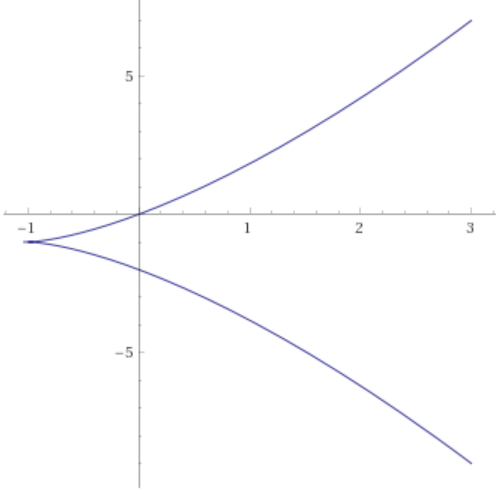
\includegraphics[scale=0.5]{xy}
    \end{subfigure}
    \begin{subfigure}{0.5 \textwidth}
        \centering
        \caption{Path $(x(t),y(t))$}
        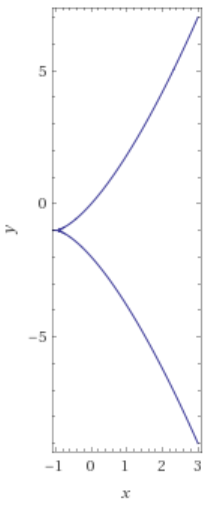
\includegraphics[scale=0.5]{f}
    \end{subfigure}
\end{figure}

\begin{tcolorbox}
c) Prove that every pair $x(t), y(t)$ of real polynomials satisfies some real polynomial relation $f(x,y)=0$.
\end{tcolorbox}

\begin{proof}

Fix polynomials $x(t)$ and $y(t)$.
Denote $n$ the higher of the degrees of $x(t)$ and $y(t)$.
Consider $W_k$, vector space of polynomials in two variables of degree at most $k$.
Monomials of degrees $0,1,\dots,k$ form a basis for the vector space of polynomials of degree at most $k$.
For a polynomial in two variables, there exist $p+1$ different monomials of degree $p$ (for example, for $p=3$ possible monomials are: $x^3, x^2y, xy^2, y^3$).
Thus, the total number of possible monomials for a polynomial in two variables of degree $k$ is
\[ \dfrac{(k+1)(k+2)}{2}. \]
This is also the dimension of $W_k$.

For every polynomial $f(x,y) \in W_k$ we can substitute $x(t)$ and $y(t)$ into $f(x,y)$, simplify and arrive at a polynomial in one variable of degree at most $nk$, which is an element of vector space $V_{nk}$ of dimension $nk+1$.
By doing so, for a given $x(t)$ and $y(t)$, we have defined a map $\varphi_{xy} :  W_k \to V_{nk}$.

We notice that $\varphi$ is a linear map.
Indeed, consider two polynomials $f,g \in W_k$:
\begin{gather*}
    \varphi(f+g) = f(x,y) + g(x,y) = \varphi(f) + \varphi(g), \\
    \varphi(c f) = c f(x,y) = c \varphi(f).
\end{gather*}

We notice that for sufficiently large values of $k$:
\begin{gather*}
    \dfrac{(k+1)(k+2)}{2} > nk, \\
    \dim W_k > \dim V_{nk}.
\end{gather*}
Therefore, by rank-nullity theorem, $\dim \ker \varphi_{xy} > 0$ and $\ker \varphi_{xy} \neq \set{0}$.
Thus, there exists non-zero polynomial $f \in W_k$ such that $\varphi_{xy}(f) = f(x(t),y(t)) = 0$.

\end{proof}


\subsection*{Problem 2}

\begin{tcolorbox}
Prove that every $m \times n$ matrix $A$ of rank $1$ has the form $A = XY^t$, where $X, Y$, are $m$- and $n$-dimensional column vectors.
How uniquely determined are these vectors.
\end{tcolorbox}

\begin{proof}

Dimension of the column-space of matrix $A$ of rank $1$ is $1$, i.e. it is a line. Therefore, any one of column vectors of $A$ is the basis of column-space of $A$. Choose one column-vector $B_i$, then all other column vectors of $A$ are multiples of $B_i$:
\[
    A = 
    \begin{bmatrix}
        | & | && | && | \\
        c_1 B_i & c_2 B_i & \cdots & B_i & \cdots & c_n B_i \\
        | & | && | && |
    \end{bmatrix}
\]
This is equivalent to:
\begin{equation} \label{eq:1}
    A = B_i C(i)^t,
\end{equation}
where
\[
    C(i) =
    \begin{pmatrix}
        c_1 \\
        \vdots \\
        c_{i-1} \\
        1 \\
        c_{i+1} \\
        \vdots \\
        c_n
    \end{pmatrix}.
\]
$B_i$ is a $m$-dimensional column vector and $C(i)$ is a $n$-dimensional column vector, as required.

\end{proof}

Since we could choose any one of column vectors of $A$ as a basis $B_i$, there exist $n$ possible combinations of $B_i$ and $C(i)$ that satisfy (\ref{eq:1}), specifically:
\[ B_i = c_i B_1, \quad \quad C(i) = \frac{1}{c_i} C(1), \]
where $c_i$ is one of entries of $C(1)$.


\subsection*{Problem 3}

\begin{tcolorbox}
a) Let $U$ and $W$ be vector spaces over a field $F$.
Show that the two operations $(u,w)+(u',w') = (u+u', w+w')$ and $c(u,w) = (cu, cw)$ on pairs of vectors make the product set $U \times W$ into a vector space.
It is called a product space.
\end{tcolorbox}

\begin{proof}

We will prove that $V$ is a vector space directly from the definition of a vector space.

We first check that $+$ makes $U \times W$ into abelian group $V^+$. Indeed, $V^+$ is the product group $U^+ \times W^+$ of abelian groups, thus it is itself an abelian group. We also note that $V^+$ includes identity $(0_U, 0_W)$.

We then check that $1v = v$, for all $v \in V$. Indeed:
\[ 1v = 1(u,w) = (1u,1w) = (u,w) = v. \]

We check the associativity of scalar multiplication. Indeed:
\[ (ab)(u,w) = (abu,abw) = a(bu,bw) = a(bv). \]

Finally, we check distributive laws. For scalar multiplication:
\begin{align*}
    (a+b)(u,w) & = ((a+b)u,(a+b)w) = (au+bu, aw+bw) \\
    & = (au,aw)+(bu,bw) \\
    & = a(u,w)+b(u,w).    
\end{align*}
For scalar addition:
\begin{align*}
    a((u,w)+(u'+w')) & = a(u+u',w+w') = (au+au',aw+aw') \\
    & = (au,aw)+(au',aw') \\
    & = a(u,w)+a(u',w')
\end{align*}

Therefore, $V$ is a vector space.

\end{proof}

\begin{tcolorbox}
b) Let $U$ and $W$ be subspaces of a vector space $V$.
Show that the map $T: U \times W \to V$ defined by $T(u,w) = u+w$ is a linear transformation.
\end{tcolorbox}

\begin{proof}

We check linearity of $T$ directly from the definition of a linear transformation:
\begin{gather*}
    T((u, w) + (u', w')) = T(u+u', w+w') = u+u'+w+w' 
    = T(u,w) + T(u',w'). \\
    T(c(u,w)) = T(cu,cw) = cu+cw = c(u+w) 
    = c T(u,w).
\end{gather*}
Therefore, $T$ is a linear transformation.

\end{proof}

\begin{tcolorbox}
c) Express the dimension formula for $T$ in terms of the dimension of subspaces of $V$.
\end{tcolorbox}

By the Rank-nullity theorem:
\[ \dim V = \dim \ker T + \dim \im T. \]

\begin{claim}
    $\dim \ker T = \dim (U \cap W)$
\end{claim}

\begin{proof}
We notice that for any $u \in U, w \in W$ the value of $T(u,w)$ is zero if and only if $u = - w$. Indeed:
\[ T(u,w) = u+w = 0 \iff u = -w. \]
This can be the case only when $u$ and $w$ are in the same subspace, i.e. $\ker T = U \cap W$.
Therefore, $\dim \ker T = \dim (U \cap W)$
\end{proof}

\begin{claim}
    $\dim \im T = \dim U + \dim W - \dim (U \cap W)$
\end{claim}

\begin{proof}
We notice that $\im T$ is the sum of all possible vectors from $U$ and $W$, i.e. $\im T = U+W$.
We know that $\dim(U+W) = \dim U + \dim W - \dim (U \cap W)$, as requested.
\end{proof}

We conclude that
\begin{align*}
    \dim V 
    & = \dim (U \cap W) + \dim U + \dim W - \dim (U \cap W) \\
    & = \dim U + \dim W.    
\end{align*}

We can double-check this result directly.
Let $\set{u_1, \cdots u_n}$ be a basis of $U$ ($\dim U = n$) and let $\set{w_1, \cdots w_m}$ be a basis of $W$ ($\dim W = m$).
Set of vectors $B = \set{(u_1,0),\dots,(u_n,0),(0,w_1),\dots,(0,w_m)}$ is linearly independent and spans $V = U \times W$. Therefore, $B$ is a basis of $V$ and $\dim V = n + m = \dim U + \dim W$.


\subsection*{Problem 4}

\begin{tcolorbox}
Let 
$
A =
\begin{bmatrix}
    a & b \\
    c & d
\end{bmatrix}
$
be a $2 \times 2$ matrix with eigenvalue $\lambda$.

a) Show that unless it is zero, the vector $v = (b, \lambda - a)^t$ is an eigenvector.
\end{tcolorbox}

\begin{proof}
\begin{equation} \label{eq:2}
    Av =
    \begin{bmatrix}
    a & b \\
    c & d
    \end{bmatrix}
    \begin{bmatrix}
        b \\
        \lambda - a
    \end{bmatrix}
    =
    \begin{bmatrix}
        ab + \lambda b - ab \\
        bc + \lambda d - ad
    \end{bmatrix}
    = 
    \begin{bmatrix}
        \lambda b \\
        \lambda d - (ad-bc).
    \end{bmatrix}
\end{equation}
We know that the characteristic polynomial for a $2 \times 2$ matrix can be expressed as follows:
\[ p(t) = t^2 - (\trace A)t + (\det A), \]
and $\lambda$ is the root of the equation $p(t) = 0$, thus:
\begin{gather*}
    \lambda^2 - (a+d)\lambda + (ad-bc) = 0, \\
    \lambda d - (ad-bc) = \lambda (\lambda - a). 
\end{gather*}
Substituting into the expression (\ref{eq:2}):
\[
    Av = 
    \begin{bmatrix}
        \lambda b \\
        \lambda (\lambda - a)
    \end{bmatrix}
    =
    \lambda
    \begin{bmatrix}
        b \\
        \lambda - a
    \end{bmatrix}
    = \lambda v.
\]
Therefore, $v$ must be an eigenvector of $A$ with eigenvalue $\lambda$.

\end{proof}

\begin{tcolorbox}
b) Find a matrix $P$ such that $P^{-1}AP$ is diagonal, assuming that $b \neq 0$ and that $A$ has distinct eigenvalues.
\end{tcolorbox}

\begin{proof}

Since characteristic polynomial $p(t)$ of $A$ is degree $2$ (see part b), $A$ has at most two eigenvalues. One of them, $\lambda$, is provided to us, and we denote another one $\lambda'$ (assume $\lambda \neq \lambda'$).

It is known that trace of a matrix is the sum of its eigenvalues. For matrix $A$ we have:
\begin{equation} \label{eq:3}
    \lambda + \lambda' = a+d.
\end{equation}
By Artin 4.6.10, matrix $\Lambda = P^{-1} A P$ is a diagonal matrix for
\[
    P = 
    \begin{bmatrix}
        | & | \\
        P_1 & P_2 \\
        | & |
    \end{bmatrix},
\]
where $P_1$ and $P_2$ are the coordinates (column vectors) of eigenvectors of $A$ in the standard basis.

As we have proved, in the Part a), eigenvectors of $A$ have the form $v = (b, \lambda - a)^t$, thus:
\begin{align*}
    v_1
    & = (b, \lambda - a)^t, \\
    v_2 
    & = (b, \lambda' - a)^t. \\
    \intertext{Substituting (\ref{eq:3}):}
    v_2
    & = (b, a+d-\lambda - a)^t = (b, d - \lambda)^t.
\end{align*}
Therefore:
\[
    P = 
    \begin{bmatrix}
        b & b \\
        \lambda - a & d - \lambda
    \end{bmatrix}.
\]

We need to make sure that $P$ is invertible:
\[ \det P = b (a + d - 2 \lambda) \neq 0. \]
Since $b \neq 0$, we just need to prove that $a+d-2\lambda \neq 0$. This is indeed the case for $\lambda \neq \lambda'$, since otherwise we would have:
\begin{align*}
    a+d & = 2\lambda \\
    \shortintertext{using (\ref{eq:3}):}
    \lambda + \lambda' & = 2\lambda, \\
    \lambda' & = \lambda,
\end{align*}
which produces a contradiction.
Thus, $P$ is invertible.
Therefore, matrix $\Lambda = P^{-1} A P$ is diagonal.

\end{proof}


\subsection*{Problem 5}

\begin{tcolorbox}
Let $v = (a_1, \dots, a_n)$ be a real row vector. We may form the $n! \times n$ matrix $M$ whose rows are obtained by permuting the entries of $v$ in all possible ways. The rows can be listed in an arbitrary order. Thus if $n=3$, $M$ might be
\[
    \begin{bmatrix}
        a_1 & a_2 & a_3 \\
        a_1 & a_3 & a_2 \\
        a_2 & a_3 & a_1 \\
        a_2 & a_1 & a_3 \\
        a_3 & a_1 & a_2 \\
        a_3 & a_2 & a_1
    \end{bmatrix}.
\]
Determine the possible ranks that such matrix could have.
\end{tcolorbox}

Rank of a matrix is the dimension of its column space and also the dimension of its row space.
Thus, rank of $A$ is at most $n$.

We explore some concrete examples.
We notice that for $v=(0,\dots,0)$, all entries of matrix $M$ are zero, thus $M$ has rank $0$.

We then notice that for $v=(a,0,\dots,0), \> a \in \R$, the set of permutations of the entries of $v$ contains linearly independent set of vectors
\[ \set{ \> (a,0,\dots,0), \> (0,a,0,\dots,0), \> \dots, \> (0,\dots,0,a) \> }. \]
In this case, rank of $A$ is $n$.

We notice that for $v=a(1,1,\dots,1), \> a \in \R$, all entries of matrix $M$ are equal to $a$, thus $M$ has rank $1$.

Now we consider a general case with at least two entries of $v$ not being equal to one another: let $v_m \neq v_k$.

Let the first row of $A$ (vector $v_e$) correspond to the original vector $v$.
Consider the row vector $v_{(mk)}$ that corresponds to the permutation $(mk)$ of $v$ (swap $m$-th and $k$-th entries of $v$).
\begin{align*}
    v_e & = (a_1, a_2, \dots, a_m, \dots, a_k, \dots, a_n), \\
    v_{(mk)} & = (a_1, a_2, \dots, a_k, \dots, a_m, \dots, a_n).
\end{align*}
Consider the following vector $p$: 
\begin{equation}\label{eq:4}
    p = \dfrac{1}{a_m-a_k} (v_e - v_{(mk)}),    
\end{equation}
which results in
\[ p = (0, \dots, 1, 0, \dots, -1, 0, \dots, 0). \]

Denote $R$ the row space of $M$.
Since $p$ is a linear combination of the rows of $M$, $p$ must be in $R$.

We notice that we could have chosen different permutations of $v$ instead of $v_1$ and $v_{(mk)}$.
Then, after (\ref{eq:4}), we would arrive at a vector that is a permutation of the entries of $p$.
In fact, we can achieve any permutation of the entries of $p$ by using the appropriate permutations of the entries of $v$.
Therefore, denoting $P$ the set of all permutations of the entries of $p$, we conclude that $P \subseteq R$.
Furthermore, since $P$ is in $R$, a vector space spanned by the vectors of $P$ must be a subspace of $R$.

Consider $P_m \subseteq P$, the set of vectors that correspond to permutations of the entries of $p$ that fix the $m$-th element of (i.e., $1$).

\begin{claim}
$P_m$ is a basis of the span of $P$.    
\end{claim}

\begin{proof}

To prove this, we first notice that set $P_m$ is linearly independent.
We also claim that every $p' \in P$ is a linear combination of vectors in $P_M$.
Let the $x$-th entry of $p'$ be $1$ and let its $y$-th entry be $-1$, then:
\[ p' = p_{(ky)} - p_{(kx)}. \]
Since both $p_{(ky)}, p_{(kx)}$ are elements of $P_m$, then $p'$ is a linear combination of elements of $P_m$.
Since every element of $P$ can be represented as a linear combination of elements of $P_m$, $P_m$ is a basis of the span of $P$.

\end{proof}

Basis $P_m$ has $n-1$ vectors, thus dimension of the span of $P$ is $n-1$.
Since $\spn P \subseteq R$, dimension of $R$ must be at least $n-1$ and, thus, $M$ has rank of at least $n-1$.

Therefore, the possible ranks of matrix $M$ are: $0,1,n-1$ and $n$.


\subsection*{Problem 6}

\begin{tcolorbox}
Determine the finite-dimensional spaces $W$ of differentiable functions $f(x)$ with this property: If $f$ is in $W$, then $\dfrac{df}{dx}$ is in $W$.
\end{tcolorbox}

We assume vector space $W$ is over field of complex numbers $\C$.
Let $n$ be dimension of $W$.

\begin{proof}

We first note that every element of $W$ must be infinitely differentiable.
Furthermore, for arbitrary function $f$ in $W$ infinite set of vectors
\[ W_f = \set*{f, \frac{df}{dx}, \frac{d^2 f}{dx^2}, \frac{d^3 f}{dx^3}, \cdots }. \]
is a subset of $W$.
Since $n$ is the dimension of $W$, every finite subset of $W_f$ with more than $n$ elements must be linearly dependent.
Consider set of vectors
\[ \set*{ f, \frac{df}{dx}, \frac{d^2 f}{dx^2}, \cdots, \frac{d^n f}{dx^n} }, \]
which must be linearly dependent.
Then there must exist some coefficients $a = \set{a_0, a_1, \dots a_n}$ such that
\begin{equation} \label{eq:5}
a_0 f + a_1 \frac{df}{dx} + a_2 \frac{d^2 f}{dx^2} + \cdots + a_n \frac{d^n f}{dx^n} = 0.
\end{equation}
Every $f \in W$ must satisfy this linear homogeneous differential equation for some coefficients $a$.
Solution space of the general equation of the form (\ref{eq:5}) has basis of
\[ B = \set*{ x^k e^{\alpha x} : k \in \N, \> 0 \leq k \leq n, \> \alpha \in \C }. \]
Therefore, any subset $B'$ of $B$ with $n$ elements, such that for every element $g \in B'$, its derivative $\dfrac{dg}{dx}$ is also in $B'$, is a basis for some space $W$.

For arbitrary $g = x^k e^{\alpha x}$ in $B'$:
\[ \frac{dg}{dx} = \frac{d(x^k e^{\alpha x})}{dx} = k x^{k-1} e^{\alpha x} + \alpha x^k e^{\alpha x}, \]
therefore functions
\[
    B_{\alpha, k} = \set*{ \>
        x^k e^{\alpha x}, \>
        x^{k-1} e^{\alpha x}, \>
        \dots, \>
        e^{\alpha x} \>
    }
\]
are in $B'$.

Every $W$ with dimension $n$ can be represented as a direct sum of subspaces, each with a basis of the form $B_{\alpha_i, k_i}$.
\[ W = \bigoplus B_{\alpha_i,k_i}, \]
such that every $\alpha_i$ is different and  $\sum k_i = n$.

\end{proof}


\subsection*{Additional Problem 1}

\begin{tcolorbox}
Let $V$ be a finite-dimensional vector space. A linear operator $T: V \to V$ is called a projection if $T^2 = T$ (not necessarily an "orthogonal projection").
Let $K$ and $W$ be the kernel and image of a linear operator $T$.
Prove

a) $T$ is a projection onto $W$ if and only if the restriction of $T$ to $W$ is the identity map.
\end{tcolorbox}

We first proof the following claim.

\begin{claim}
Any surjective operator $P : U \to U$ is invertible.
\end{claim}

\begin{proof}
By the rank-nullity theorem:
\begin{gather*}
    \dim U = \dim \ker P + \dim \im P, \\
    \dim U = \dim \ker P + \dim U, \\
    \dim \ker P = 0,
\end{gather*}
therefore, any surjective operator is invertible.
\end{proof}

We proceed with the proof of the problem.

\begin{proof}
($\Longrightarrow$):
Suppose $T^2 = T$ on $V$, then $T^2\restrict{W} = T\restrict{W}$.
Map $T\restrict{W}: W \to W$ is a surjective operator, thus invertible.
Left multiplying $T^2\restrict{W} = T\restrict{W}$ by $\left(T\restrict{W}\right)^{-1}$ we have $T\restrict{W} = I$, as requested.

($\Longleftarrow$):
Suppose $T \restrict{W} = I$.
Since image of $T$ is $W$, we have $T^2 = T\restrict{W}T = T$, as requested.

\end{proof}

\begin{tcolorbox}
b) If $T$ is a projection, then $V$ is the direct sum $W \oplus K$.
\end{tcolorbox}

\begin{proof}

Consider $v$, an arbitrary element of $W \cap K$.
Then $v$ is in the image of $T$, we have $Tv = v$.
Since $v$ is in the kernel of $V$, we have $Tv = 0$.
We conclude that $v = 0$ and $W \cap K = \set{0}$.

Since intersection of $W$ and $K$ is zero and by the rank-nullity theorem, we have
\[ \dim (W+K) = \dim W + \dim K = \dim V. \]
Since $W+K$ are subsets of $V$ and dimension of their sum $W+K$ is equal to the dimension of the space $V$ itself, we conclude that $W+K$ spans $V$.
Since $W \cap K = \set{0}$, we have that $V$ is a direct sum of $W$ and $K$, as requested.

\end{proof}

\begin{tcolorbox}
c) The trace of a projection $T$ is equal to its rank.
\end{tcolorbox}

\begin{proof}

Suppose $V$ has dimension $n$ and suppose projection $T$ has rank $m$.
Choose arbitrary basis of $W$, denote it $\set{w_1, \dots, w_m}$.
We can extend this basis to the basis of $V$:
\[ B = \set{w_1, \dots, w_m, k_1, \dots, k_{n-m}}. \]
By part b) of the problem, $W \oplus K = V$, therefore each $k_i$ must be an element of $K$.
Then, each $k_i$ is in the kernel of $T$, therefore $T k_i = 0$.
Since each vector $w_i$ is in the image of $T$, by part a) of the problem, we have that $T v_i = v_i$.

Matrix representation of $T$ with regards to basis $B$ will have the following form:
\[
    \begin{pmatrix}
        1 \\
        & \ddots \\
        & & 1 \\
        & & & 0 \\
        & & & & \ddots \\
        & & & & & 0
    \end{pmatrix}
\]
with $m$ ones and $n-m$ zeroes on the diagonal.
Such matrix has trace $m$. Therefore $T$ has trace $m$ equal to the rank of $T$, as required.

\end{proof}


\end{document}
